\section{Introduction}
\label{sec:intro}

Data exploration is the act of querying a database to discover its content.
Ultimately, the aim is to discover \emph{nuggets}, i.e., interesting queries
that expose unexpected phenomena.  Because this task
is important and omnipresent, engineers have devised \emph{exploration
systems} to support it. These systems let users ``play'' with their tuples. They
provide facilities to write queries and visualize the results quickly.
They engage their users in a loop of trial and errors, through which they discover
their data. Examples of such systems are Tableau~\cite{StolteTangHanrahan2002},
based on visualizations, Blink~\cite{agarwal2012blink}, based on sampling, or
Blaeu~\cite{sellamTKDE} based on clustering.

Exploration systems assume that users can evaluate the usefulness of a set of
tuples simply by looking at it - or at least, by looking at a sample.
Typically, they present the results of the queries with tables, visualizations,
or statistical summaries, in the hope that users will know what to inspect and
where to go next. And indeed, this assumption holds with low dimension data.
If a set of tuples involves less than a dozen columns, the users can plot it,
build a mental picture of what it contains and judge whether they effectively
found a nugget or not. But the assumption breaks down in high dimension spaces.
If the query results contains dozens or hundreds of columns, which ones should the users
inspect? The resulting tuples are overwhelmingly large.  Our explorers may not be able to
recognize the nugget they had been wishing for even if it appeared on their
screen.  

One approach to solve this problem is to use dedicated multidimensional
visualization methods, such as scatter-plot matrices or parallel coordinates.
But these methods cannot scale to the volumes we envision. For example, a
scatter plot matrix would require at least 190 distinct plots to represent a
simple dataset with only 20 columns - this is hardly a progress compared to
tables.

An alternative approach is to apply dimensionality reduction algorithms to the
user's selection, such as Principal Component Analysis.  But these methods
transform the data: they rescale it, project it and rotate it.  Therefore, the
tuples that the users visualize are not those that they requested in the first
place.  Furthermore dimensionality reduction techniques ignore the exploration
context: they compress the user's selection, but they do not show how it
compares to the rest of the database. Hence, they may miss interesting
aspects of the selection.

In this demo proposal, we introduce Ziggy, a system to help explorers
understand the results of their queries.  Ziggy detects and plots
\emph{characteristic views}, that is, small sets of columns on which the user's
tuples are different from those in the rest of the database.  By consulting
these views, our explorers can understand what makes their selection
``special'' and steer the exploration accordingly. 

Our system can detect informative views, but it can also \emph{justify} its
choices.  For each view, it generates a short paragraph which explains why it
chose these columns.  While several existing papers have presented mechanisms
to query databases in natural language, little to none of them have tackled the
reverse direction: how to describe the results in plain English. Our system
pioneers this field.

This demonstration will introduce the tuple characterization problem,
previously described in a full research paper\footnote{At the time of writing,
the paper was under review at VLDB.}.  The visitors will discover real-life
datasets and experiment with Ziggy's engine.  Eventually, the demo will show
that our prototype can extract surprising insights from datasets of all levels
of complexity.
\pagebreak

\section{Characterizing Tuples}
\label{sec:overview}

Let us present Ziggy with an example. An analysts wants to understand what
causes violent crimes in US cities. She has access to a large table, containing
130 economic, social and demographic indicators for a few thousand communities. To
seed the exploration, she selects the cities with the highest rates of
criminality. Her database front-end returns a large table with more than a
hundred columns. Which ones should she inspect?

\begin{figure}[t!]
    \centering
    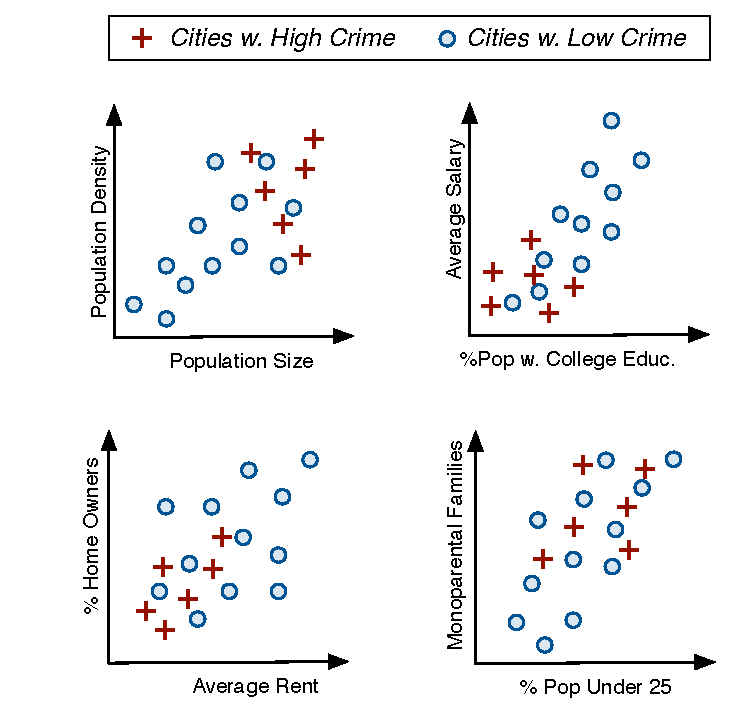
\includegraphics[width=.9\columnwidth]{Images/CharacViews}
    \caption{Four examples of characteristic views.}
    \label{fig:characteristic-views}
\end{figure}

Ziggy addresses the problem in two steps. First, it presents several
low-dimension views of the database, which highlight the differences between
the tuples in the query results and those in the remainder of the database.
Figure~\ref{fig:characteristic-views} depicts four of these views.  On all four
plots, we observe that the selection has an unusual statistical distribution
compared to the other tuples. The first plot shows that cities with a high
crime index tend to have particularly high densities and large populations. In
the second view, we see that these cities correspond to low levels of
education.  The third view reveals that dangerous neighbourhoods tend to have
lower rents and a lower percentage of home ownership. The last one reveals that
they are generally younger, with more mono-parental families.

In a second step, Ziggy \emph{explains} its choices. Indeed, our system can
veritably motivate its decisions, using natural language. For instance, it
would comment the first view of Figure~\ref{fig:characteristic-views} as
follows:
\begin{quotation}
    ``On columns~\texttt{Population} and \texttt{Density}, your selection has
    particularly high values and a low variance''
\end{quotation} 
This short paragraph describes why Ziggy chose the columns \texttt{Population}
and \texttt{Density}. The users can interpret these explanations as hints for
further exploration, to make sure that they have not missed any 
aspect of their query results. Alternatively, they can use them for sanity
checks, to control the correctness of Ziggy's views.

\section{Problem Formulation}
\label{sec:algorithm}

%Evidently there are a plethora of use cases that would fit this intuition and be aided by
%a system along these lines. The challenge is to turn it into a working system.
%We gave an intuitive overview characteristic views and we explained why they
%were useful. 
We described the intuition behind characteristic views.  The challenge is now
to turn it into a working system. In this section, we formalize our problem: we
present Ziggy's objective function, and we describe how it scores the views.

\subsection{General Statement} 
When seeking views, Ziggy must consider two aspects. It must first find columns
on which the users' selection have an unusual statistical distribution.
Thereafter, it must enforce that its views are not redundant with each other.
Let us formalize these objectives.

\label{sec:problem}
\begin{figure}[t!]
    \centering
    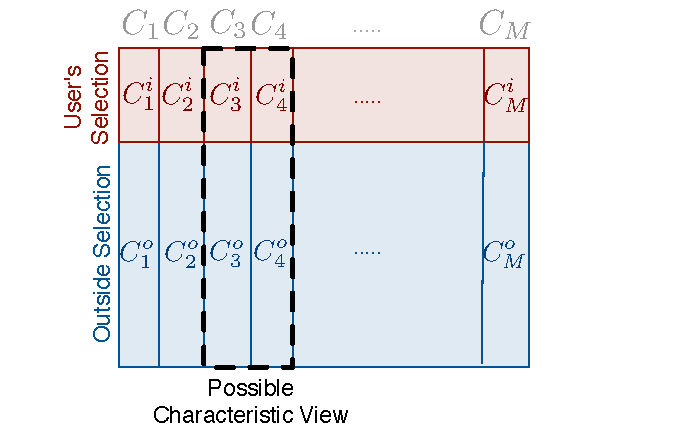
\includegraphics[width=0.75\columnwidth]{Images/Setting}
    \caption{Our problem setting.}
    \label{fig:setting}
\end{figure}
Let the random variables $C_1, \ldots, C_M$ represent the columns in the
database.  We assume that the variable $C_j^i$ represent the tuples covered by
the selection, and that $C_j^o$ represents the tuples outside the selection, as
shown in Figure~\ref{fig:setting}.  Ziggy's aim is to find a set of at most $D$
columns such that the distribution of $C_1^o, \ldots, C_D^o$ is as different as
possible from that of $C_1^i, \ldots, C_D^i$. If $\mathfrak{D}$ represents a
measure of statistical divergence from the statistics literature, our aim is to
find the top views $\mathcal{V}_i = \{C_1, \ldots, C_D\}$ that maximize the
following quantity:
\begin{equation}
    \label{eq:objective0}
    \text{score} (\mathcal{V}_i) = \mathfrak{D}\big( C_1^o, \ldots, C_D^o \,;\, C_1^i, \ldots, C_D^i \big)\\
\end{equation}
Common examples of divergence functions $\mathfrak{D}$ are the distance between
the centroids and the Kullback-Leibler divergence~\cite{wasserman2013all}.  We
will present our own in the next subsection.

Equation~\ref{eq:objective0} is not complete because it leads to
redundancy: a small number of columns may appear in all the best views. To
control this effect, we introduce a constraint in our problem.  Assume
that we have already discovered $i-1$ views $\mathcal{V}_1, \ldots,
\mathcal{V}_{i-1}$. Let the notation $\mathcal{V}_{1 \ldots i-1}$ describe
their union, i.e., $\mathcal{V}_{1 \ldots i-1} = \bigcup_{v \in [1,i-1]}
\mathcal{V}_v$. For some user-defined integer $L$, our aim is to find a new
view $\mathcal{V}_i$ that solves the following optimization problem:
\begin{equation}
    \label{eq:objective}
    \begin{aligned}
        \text{Argmax}_{\mathcal{V}_i}\; 
        & \text{score} (\mathcal{V}_i)\\
         \text{s.t.} 
         & \left|\mathcal{V}_{1\ldots i-1} \cap  \mathcal{V}_i  \right| \leq L\\ 
    \end{aligned}
\end{equation}
The constraint enforces view diversity: it makes sure that that the new view
$\mathcal{V}_i$ borrows at most $L$ columns from the precedent views.
\pagebreak

\subsection{Dissimilarity Measure}
The statistics literature presents many options to instantiate the statistical 
divergence measure $\mathfrak{D}$~\cite{wasserman2013all}. But most of those
operate in a ``black box'' fashion: they indicate how much two distributions
differ, but they do not explain why. We now introduce our own function, the
\emph{Zig-Dissimilarity}, that overcomes this problem.

\begin{figure}[t!]
    \centering
    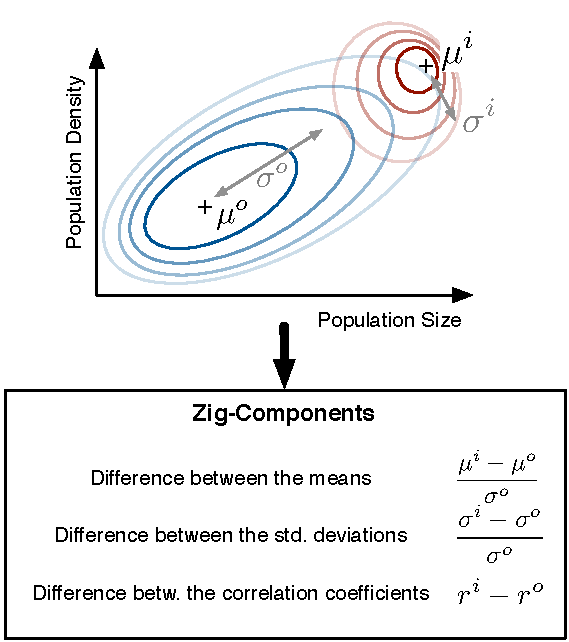
\includegraphics[width=.85\columnwidth]{Images/Zig-Dissimilarity}
    \caption{Examples of Zig-Components.}
    \label{fig:zig-dissim}
\end{figure}

The main idea behind the Zig-Dissimilarity is to  compute several simple
indicators of dissimilarity, the \emph{Zig-Components}, and aggregate them into
one synthetic score.  Figure~\ref{fig:zig-dissim} presents three such
indicators: the difference between the means, the difference between the
standard deviations and the difference between the correlation coefficients. We
see that each Zig-Component highlights one particular ``aspect'' of the
difference between the distributions.  Also, these functions are verifiable:
the users can inspect the charts and check whether they hold.  Most of our
Zig-Components come from the statistics literature, where they are referred to
as \emph{effect sizes}~\cite{hedges2014statistical}. Observe that we test
dissimilarities in spaces with one but also two dimension. For instance, the
difference between the correlation coefficients involves two dimensions. In
principle, we could design Zig-Components for higher dimensionalities.
Nevertheless, practice revealed that those only add a marginal accuracy gains,
at the cost of significant processing times. Also, we ignore the Zig-Components
for categorical data - we discuss them in our full paper.

To aggregate the Zig-Components, we normalize them and compute a weighted sum.
The normalization enforces that the indicators have comparable scale. The
weights in the final sum are defined by the user. Thus, they can express their
preference for one type of difference over the others. 

\section{Ziggy's Architecture}
\label{sec:solution}

The next step is to build a system to solve the problem raised.
%We formalized the multi-view characterization problem. We now present how Ziggy
%solves it.
Figure~\ref{fig:architecture} presents Ziggy's tuples description pipeline.  It
includes three stages: preparation, view construction and post-processing.
During the preparation stage, Ziggy collects the statistics necessary to build
the views. In the View Construction stage, it effectively forms the views.
During the last step, it checks if the views are statistically robust and it
generates the justifications.
\begin{figure}[t!]
    \centering
    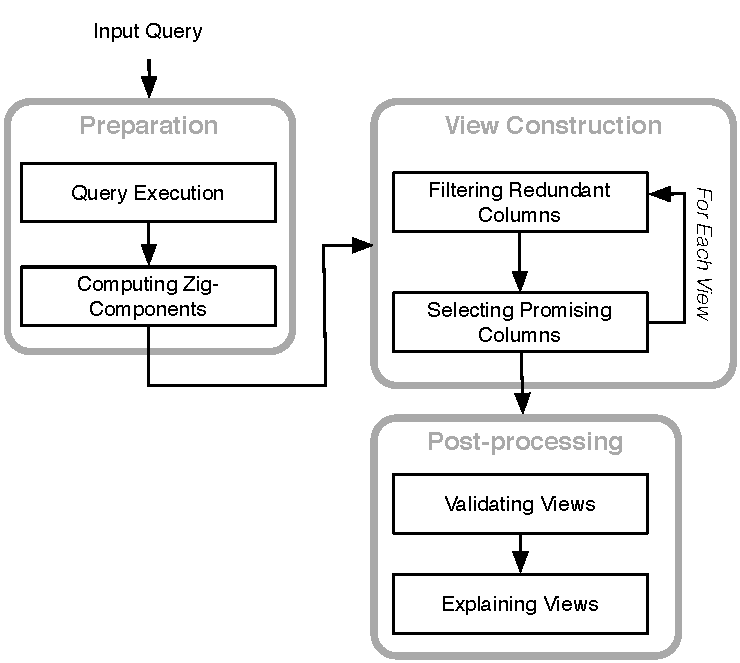
\includegraphics[width=\columnwidth]{Images/Algorithm}
    \caption{Ziggy's Tuples Description Pipeline.}
    \label{fig:architecture}
\end{figure}

\vfill
\textbf{Preparation.} During the preparation step, Ziggy executes the user's
query, loads the results, and computes the Zig-Components associated to each
column and each couple of columns. This step is by far the most time consuming.
In our manuscript, we present a strategy to share computations between queries,
and therefore reduce the amount of data to read. The output of these operations
is a table, which describes the Zig-Components associated to each variable and
each pair of variables.

\vfill
\textbf{View Construction.} In this step, Ziggy builds the views one by one, in
a greedy manner. It operates as follows. First, it detects which columns
violate the redundancy constraint of Equation~\ref{eq:objective}, and it
discards them. Then, it detects the pairs of columns associated to the highest
Zig-Components, and it appends them to the view. It stops building views when
it has processed all the columns in the database, or when the
Zig-Dissimilarities are too weak for the results to be statistically
significant (cf.  next step).

\vfill
\textbf{Post-Processing.} During the final phase, Ziggy evaluates the
statistical robustness of the views. The aim is to control spurious findings,
that is, differences caused by chance. For each view, it tests the
significance of the Zig-Component separately, using asymptotic bounds from the
literature~\cite{hedges2014statistical}. Then it aggregates the confidence
scores associated to each component. Depending on the users' preferences, it
retains the smallest value, or it uses more advanced aggregation schemes such
as the Bonferroni correction~\cite{wasserman2013all}. 

During the last step, Ziggy also generates the explanations. Given the
composite nature of the Zig-Dissimilarity, this step is straightforward: Ziggy
choses the Zig-Components associated with the highest level of confidence, and
it describes them with text. We implemented the text generation functionalities
with hand-written rules.
\begin{figure*}[!th]
    \centering
    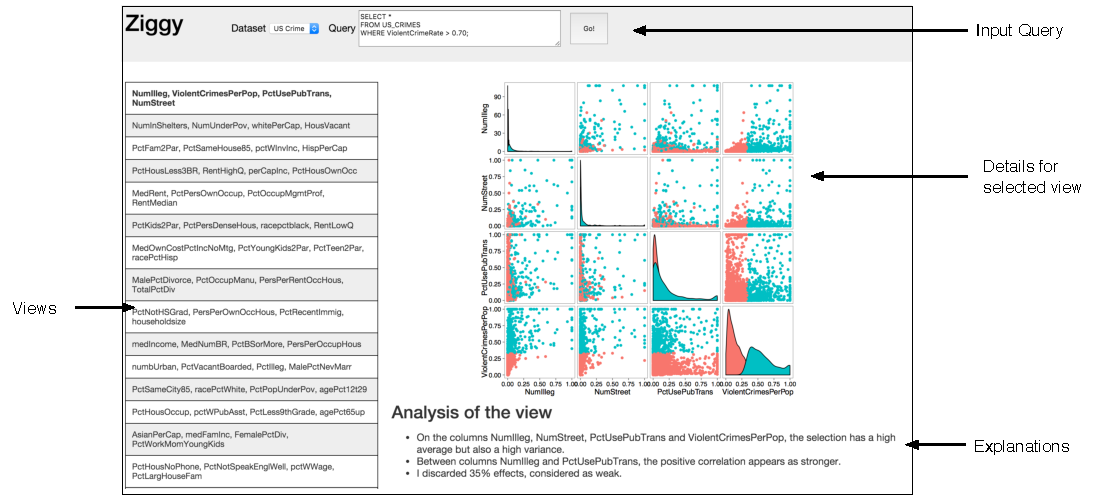
\includegraphics[width=.95\textwidth]{Images/ScreenDetail}
    \caption{Snapshot of Ziggy's interface.}
    \label{fig:screenshot}
\end{figure*}
\pagebreak


\section{Implementation and Demo}
\label{sec:demo}

\subsection{Overview of the System}
\label{sec:archi}
Our demonstration system comprises three components. In the bottom layer, a
DBMS stores and delivers the data (we chose MonetDB). The middle layer
comprises the tuple characterization engine and a Web server. We developed both
components in R, except for a few critical operations written in C (those
related to computing Zig-Components). The Web server relies on the package
\texttt{Shiny}. The front end is based on HTML and Javascript. 

Figure~\ref{fig:screenshot} presents a screenshot of our demonstration system.
Users specify their queries in the text box of the top panel. Ziggy returns the
views on the left side, ranked by decreasing order of dissimilarity.  It
displays the explanations on the right side.

\subsection{Use Cases}
\label{sec:usecases}

We will demonstrate Ziggy with three real-life datasets.
\begin{itemize0}
    \item The \textbf{Box Office} dataset describes Hollywood movies released
        between 2007 and 2013. We will use it to introduce the main concepts behind
        Ziggy: the tuple description problem, how Ziggy choses views and how to
        read them. The data contains 900 tuples and 12 columns.
    \item The \textbf{US Crime} database contains 128 crime and socio-economic
        indicators for 1994 US Cities. The dataset is freely available on the
        UCI Repository\footnote{\url{https://archive.ics.uci.edu/ml/datasets/Communities+and+Crime}}.
        The use case is similar to the running example used throughout this
        paper. We hope to surprise our visitors by showing that seemingly
        unrelated variables can have a strong predictive power - such as the
        number of boarded windows in a given neighborhood.
    \item The \textbf{Countries and Innovation} dataset describes innovation
        and patents for different regions of the world. We obtained it by
        combining different tables from the Website of the OECD, an international
        economic organization\footnote{\url{http://stats.oecd.org/}}. It
        contains 6,823 rows and 519 columns. We will show that Ziggy can
        highlight complex phenomena, in effect generating hypotheses for future
        exploration.
\end{itemize0}
During our presentation, we will use ready-made queries and encourage the
visitors to suggest their own.

\section{Conclusion}
\label{sec:conclusion}
During the last few years, authors have introduced dozens of methods to
discover new, interesting queries. In this paper, we tackled the complementary
problem: once our users have a query, how do they know if it is a good one?
Our short term objective to demonstrate Ziggy and let visitors challenge our
system. On the long term, we intend to distribute our tuple description engine
as a library, to be included into external exploration systems.

